%&spell
\section{Physics beyond the Standard Model}

Despite its countless successes, there are a plethora of indications --- both
theoretical and experimental --- that additional physics exists, beyond the SM (BSM).

\subsection{Evidence for physics beyond the Standard Model}
%%%%%%%%%%%%%%%%%%%%%%%%%%%%%%%%%%%%%%%%%%%%%%%%%%%%%%%%%%%%%%%%%%%%%%%%%%%%%%%%%%%%%%%%%%%%%%%%%%%
% Experimental
%%%%%%%%%%%%%%%%%%%%%%%%%%%%%%%%%%%%%%%%%%%%%%%%%%%%%%%%%%%%%%%%%%%%%%%%%%%%%%%%%%%%%%%%%%%%%%%%%%%
One experimental phenomena that points to \np is the observed baryon asymmetry of the Universe, and
the fact that it cannot be explained by the SM.
The amount of CP violation from the phase in the CKM matrix comes up short by approximately ten
orders of magnitude~\cite{Cline:2006ts,Huet:1994jb}.
Also, the total mass of luminous matter constitutes less than $5\,\%$ of the
total mass in the Universe, hinting at the existence of Dark Matter.
This is evidenced by flat rotation
curves~\cite{1970ApJ...159..379R,1980ApJ...238..471R} and the gravitational lensing around massive
objects, such as the Bullet Cluster~\cite{Markevitch:2003at}.
Furthermore, the SM cannot explain massive neutrinos, which are necessary to explain neutrino
oscillations, which were first observed unambiguously at
Super-Kameokande~\cite{PhysRevLett.81.1562}.



The largest tension in the \ut is in  the measurements of \V{ub}.
A determination of \V{ub} can be made using inclusive and exclusive measurements of
$\decay{B}{X_u\ell\bar\nu_\ell}$ decays.
Inclusive measurements are made difficult from large
$\decay{B}{X_c\ell\bar\nu_\ell}$ backgrounds, while exclusive semi-leptonic modes suffer from
uncertainties introduced by form factors.
A value of $\left|\V{ub}\right|$ can also be obtained from the annihilation decay
$\decay{\Bp}{\taup\nu_\tau}$ which has low statistics.
Determinations of \V{ub} from these sources are:
\begin{align}
  |\V{ub}| &= \big(4.41\,^{+0.21}_{-0.23}\big)\e{-3}, & \quad\big(\mathrm{exclusive}\big)\text{\cite{PDG2014}}& \nonumber\\
  |\V{ub}| &= \big(3.28\pm{0.29}\big)\e{-3},  & \big(\mathrm{inclusive}\big)\text{\cite{PDG2014}}&\nonumber\\
  |\V{ub}| &= \big(4.22\pm{0.42}\big)\e{-3},  & \big(\decay{\Bp}{\taup\nu_\tau}\big)\text{\cite{PDG2012}}&\nonumber\\
  %|\V{ub}| &= \big(4.22\pm{0.42}\big)\e{-3}  & \big(\decay{\Bp}{\taup\nu_\tau}\big)\text{\cite{{PhysRevD.88.031102}&\nonumber
  \label{eq:th:vub}
\end{align}
limits on \ut measurements are shown in \Fig{fig:th:ut}.
There are obvious tensions between the inclusive and exclusive modes, which could hint at some new
process.
A more accurate value of \V{ub} from the decay $\decay{\Bp}{\taup\nu_\tau}$ might shed light on the
situation.


Put in here?:
\begin{itemize}
  \item $P_5^\prime$
  \item Hyper-CP
\end{itemize}


%%%%%%%%%%%%%%%%%%%%%%%%%%%%%%%%%%%%%%%%%%%%%%%%%%%%%%%%%%%%%%%%%%%%%%%%%%%%%%%%%%%%%%%%%%%%%%%%%%%
% Theoretical
%%%%%%%%%%%%%%%%%%%%%%%%%%%%%%%%%%%%%%%%%%%%%%%%%%%%%%%%%%%%%%%%%%%%%%%%%%%%%%%%%%%%%%%%%%%%%%%%%%%
Theoretical reasons suggesting BSM physics
are often rather subjective, and revolve around the idea of natrualness.
Naturalness is a concept whereby a theory is deemed to be natural, or more plausible, if it has few
free parameters, all of which are of order one.
The SM is not a natural theory.

There are a total of 18 free parameters in the SM, 13 of which reside in the flavour sector.
The CKM matrix in $\Lag{\it q}^\mathrm{CC}$ exhibits a strongly hierarchic structure, favouring
flavour conserving weak interactions.
%This can not be explained naturally.
Neither can the range of quark masses, which vary by four orders of magnitude.

Unnatural models with parameters which differ wildly in magnitude tend to result in fine-tuning.
This is when some parameters, or process, must cause a cancellation to extremely high precision in
order to agree with experimental observations.
For example, quantum loop corrections to the Higgs mass are of the order $10^{19}$ for Higgs mass
of $\sim125\gev$~\cite{Chatrchyan:2012ufa,Aad:2012tfa}.
This means that the cancellations required to achieve a mass comparable to the masses of the weak
vector bosons must be exact to 17 orders of magnitude.
This is known as the \emph{hierarchy problem}.
Additional particles from NP would alter the amount of fine tuning required, making the model more
natural.

Fine tuning also appears in QCD.
A gauge invariant term that can be added to \Lag{QCD} is
\begin{equation}
  \Lag{QCD}^\theta = \theta\frac{g^2}{32\pi^2}
  F_{\mu\nu}^\alpha\widetilde F^{\mu\nu}_\alpha,
\end{equation}
where $\theta$ and $g$ are constants, and $\alpha$ indicates a sum over colours.
The operator $F_{\mu\nu}$ is the gluon field strength tensor, and
\begin{equation}
  \widetilde F^{\mu\nu}_\alpha = \frac12\varepsilon_{\mu\nu\rho\sigma}F^{\rho\sigma}_\alpha.
\end{equation}
An interaction such $\Lag{QCD}^\theta$ would conserve charge symmetry, but violate parity and time
conjugation~\cite{Peccei:2006as}.
Such symmetry violations are in contradiction with the observed properties of the strong
force.
Bounds placed on the value of the neutron dipole moment, $|d_n| <2.9\e{-26}\,\mathrm{ecm}$
(at 90\% CL)~\cite{Baker:2006ts} requires $\theta$ to be very small,
$\theta<10^{-19}$~\cite{Crewther:PQref9}, when \emph{a priori} it could be in the range
$0<\theta<2\pi$.
This occurrence of fine tuning is referred to as the \emph{strong CP problem}.
A solution to this problem is to introduce an additional chiral symmetry, such that $\theta$
becomes a field, the quanta of which are called axions.
%The axion model is discussed in more detail in \Sect{sec:db:theory}.



\subsection{Manifestation of physics beyond the SM}
\label{sec:th:bsm:man}

The most general way to parameterize NP is with an effective Lagrangian describing generic
interactions at an energy scale $\mu$, in which long and short distance effects are separated.
Long distance (equivalently low energy) effects are described by coefficients, $c$, which can be
calculated using perturbative methods.
Short distance (or high energy) effects are characterized by terms of operators, $\mathcal{O}$,
which must be calculated non-peturbativly because they contain QCD interactions.
The resulting effective Lagrangian includes a sum over all processes, $i$, which contribute at a
given dimension, $d$:
\begin{equation}
  \Lag{eff}
  =
  \Lag{SM} + \sum_d\frac1{\Lambda^{d-4}}
  \sum_ic_i^{(d)}\mathcal{O}_i^{(d)}.
  \label{eq:th:lageff}
\end{equation}
Processes that cause FCNCs contribute in $d=6$, and can be written as
\begin{equation}
  \Delta\mathcal{L}^\mathrm{FCNC}
  =
  \sum_{i\neq j}\frac{c_{ij}}{\Lambda^2}
  \left(\Xbar{\mathcal{O}}_{Li}\gamma^\mu\mathcal{O}_{Lj}\right)^2,
\end{equation}
where $c_{ij}$ are dimensionless FCNC couplings, where $i$ and $j$ are different quark generations.
Bounds set on the energy scale $\Lambda$ by the analysis in \Ref{Isidori:2010kg} are:
\begin{equation}
  \Lambda > \frac{|c_{ij}|^\frac12}{|\Vconj{ti}\V{tj}|}\times4.4\tev
  \sim
  \left\{
    \begin{array}{l}
      |c_{sd}|^\frac12\times 1.3\e{4}\tev \\
      |c_{bd}|^\frac12\times 5.1\e{2}\tev \\
      |c_{bs}|^\frac12\times 1.1\e{2}\tev \\
    \end{array}\right.
\end{equation}
These values are calculated under the assumption that NP has a natural flavour structure, where
$c_{ij}\sim\mathcal{O}(1)$.
So, either couplings are of order unity and NP begins to contribute at over $100\tev$; or couplings
strengths are $\mathrm{O}(10^{-5})$ and NP contributes at the $1\tev$ level;
it is expected for NP to appear at the $1\tev$ scale in order to solve the hierarchy problem.
Either way, there is a conflict between the most natural coupling and energy scale; this is known
as the \emph{flavour problem}.
This leads to a host of contradictions, leading to the conclusion that NP has a highly non-generic
flavour structure.

%The most pessimistic solution to the flavour problem is Minimal Flavour Violation (MFV)
%which simply assumes that beyond SM physics follows a Yukawa coupling like structure in the flavour
%sector, this would lead to no discernible new physics in the flavour sector.

The effective Hamiltonian for the FCNC $\decay{b}{s\ell^+\ell^-}$ is given by:
\begin{equation}
  \Ham{eff} = -4\frac{G_F}{\sqrt{2}}\Vconj{ts}\V{tb}\frac{e^2}{16\pi^2}
  \sum_{i}\big(c_i(\mu)\mathcal{O}_i(\mu)+c_i(\mu)^\prime\mathcal{O}_i^\prime(\mu)\big)
\end{equation}
similar to \Eq{eq:th:lageff}, where the coefficients are known as Wilson coefficients, which
correspond to the Wilson operators $\mathcal{O}_{1-10}$.
The operators $\mathcal{O}_{1-6}$ are sensitive to long distance contributions such as \ccbar
loops.
Operators which are particularly sensitive to NP contributions in \decay{b}{s\mumu} transitions are
\begin{align}
  \Op{7\pz} &= \frac{m_b}{e}\big(\bar s \sigma_{\mu\nu}P_Rb\big)F^{\mu\nu}
  &\Op{7\pz}^\prime &= \frac{m_b}{e}\big(\bar s \sigma_{\mu\nu}P_Lb\big)F^{\mu\nu}
  \nonumber\\
  %\mathcal{O}_8 &= g\frac{m_b}{e^2}\big(\bar s \sigma_{\mu\nu}T^aP_Rb\big)G^{\mu\nu a}
  %&\mathcal{O}_8^\prime &= g\frac{m_b}{e^2}\big(\bar s \sigma_{\mu\nu}T^aP_Rb\big)G^{\mu\nu a}
  %\\
  \Op{9\pz} &= \big(\bar s\gamma_\mu P_Lb\big)\big(\bar\ell\gamma^\mu\ell\big)
  &\Op{9\pz}^\prime &= \big(\bar s\gamma_\mu P_Rb\big)\big(\bar\ell\gamma^\mu\ell\big)
  \nonumber\\
  \Op{10} &= \big(\bar s\gamma_\mu P_Lb\big)\big(\bar\ell\gamma^\mu\gamma_5\ell\big)
  &\Op{10}^\prime &= \big(\bar s\gamma_\mu P_Rb\big)\big(\bar\ell\gamma^\mu\gamma_5\ell\big)
  \phantom{\frac{1}{1}}
  %\\
  %\mathcal{O}_{S} &= \frac{m_b}{m_{B_s}}\big(\bar s\gamma_\mu P_Rb\big)\big(\bar\ell\ell\big)
  %\\
  %\mathcal{O}_{P} &= \frac{m_b}{m_{B_s}}\big(\bar s\gamma_\mu P_Rb\big)\big(\bar\ell\gamma_5\ell\big)
\end{align}
where $P_{L,R}$ are the left and right projection operators.
The operators \Op{7} and \Op{9} describe the emission of a photon or $Z$ from a penguin loop,
and \Op{10} corresponds to a box type diagram with \Wp; these are shown in \Fig{fig:hhh:loops}.
Primed operators are the suppressed helicity, whose contributions are vanishingly small in the SM.

\begin{figure}
  \begin{center}
    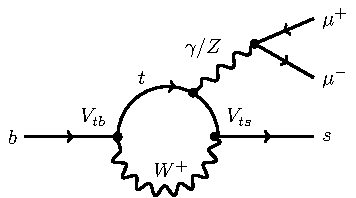
\includegraphics[scale=1]{feynman_btosmumu_penguin}
    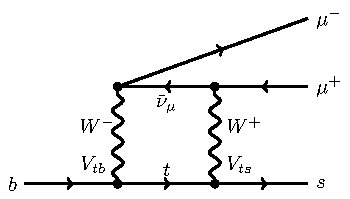
\includegraphics[scale=1]{feynman_btosmumu_box}
    \caption[Schematic Feynman diagrams for loop and box diagrams]
    {\small
      Schematic Feynman diagrams for the
      (left) penguin loop diagrams corresponding to the operators \Op{7} and \Op{9} depending on
      whether a $\gamma$ or $Z$ is emitted from the loop;
      (right) \Op{10} box diagram mediated by \Wp bosons.
    }
    \label{fig:hhh:loops}
  \end{center}
\end{figure}

As well as in loops, virtual particles can also contribute in some tree level diagrams.
The small value of $|\V{ub}|$ means that annihilation decays of \Bp mesons are heavily
suppressed in the SM.
%They are mediated by
%Tree level diagrams in the SM are typically high statistics modes, however annihilation type decays
%are heavily suppressed.
These rare modes are propagated by a \Wp in the SM; but this could be exchanged for any charged
boson, such as an $H^+$ from SUSY, this could alter the branching fraction or
introduce significant CPV.
%The decay \btodsphi is an annihilation decay of the \Bp.

New physics models must be able to accommodate Dark Matter.
Some models have a \emph{dark} or \emph{hidden} sector which, apart from gravity, only
communicates with the visible sector feebly via messenger particles.
These messenger particles could potentially be observed after they decay into SM particles after
mixing with a $H$ or $Z$.
The axion could be such a particle, as could the inflaton or dark $Z$; models including these
particles are further detailed in \Sec{sec:db:intro}.

%Dark Matter is the lightest supersymmetric particle which is stable and messenger particle is super
%goldstino
Supersymmetry (SUSY) is a theory which introduces an additional super-particle for each SM fermion and
gauge boson, whose spin is different by a half integer.
The Higgs sector in SUSY comprises four Higgs doublets; two are spin-0 and two are spin-$\tfrac12$,
and then there are two each for $Y=\pm\tfrac12$.
After SUSY is broken there are five Higgs physical scalar particles, two are CP-even ($h^0$,
$H^0$) one is CP-odd scalar ($A^0$) and two charged are charged ($H^\pm$).
Supersymmetry supplies a Dark Matter candidate in the shape of the lightest supersymmetric
particle, which could communicate with the visible sector via a super-golstino.
It also immediately solves the hierarchy problem.
The masses of the super-particles are unconstrained, and could be anywhere between a few TeV and
the Planck scale.
%The theory of SUSY immediately solves the hierarcy problem and provide a candidate for Dark Matter
%in the shape of the lightest supersymmetric particle.
%Super-goldstino
%The messenger particles are super goldtinos that arise from the breaking of the symmetry,
%However, the scale of the masses of the new particles are undefined, meaning
%they could appear anywhere from a few TeV up to the Planck scale.


The most pessimistic solution to the flavour problem is Minimal Flavour Violation (MFV)
which simply assumes that beyond SM physics follows a Yukawa coupling like structure in the flavour
sector, this would lead to no discernible new physics in the flavour sector.
Assuming that nature has not chosen MFV, then contradictions from flavour problem indicate that NP
searches should be made for both: particles
with high mass, and particles which have small coupling strengths.
The \lhcb experiment can probe the mass scale, since precision measurements of tree and loop
diagrams are sensitive to virtual particles contributing at all orders, whose on-shell mass could
be many TeV.
The relatively high luminosity of interactions supplied by the \lhc mean that \lhcb is also
sensitive to low coupling strengths, such as messenger particles from the dark sector.
The following chapters explore a variety of different searches for beyond Standard Model physics.



%Looking for NP in precision measurements from tree and loop diagrams is often referred to as
%\emph{indirect} seraches, since the source of NP is inferred.
%The other option is to search for \emph{direct} evidence of NP, such as in the invariant mass spectrum of
%a combination of particles.


%The tree level diagram \btodsphi is an annihilation type decay which is propagated by a \Wp in the
%SM.
%Additional physics could

%Contributions to physical observables from NP can alter them

%There are many indications that NP will manifest itself in the flavour sector, making in an
%excellent environment in which to search for deviations from the SM.

%It is unknown how NP will manifest itself...
%Look in different places

%\lhcb particularly looks for indirect evidence of NP.
%Rather than looking directly for an excess in an invariant mass spectrum of some particles, it is
%possible to infer the existence of NP from deviations between SM theory and measurements.

%These measurements could be made in leading leading order, tree level, diagrams.
%Chapter~\ref{ch:dsphi} details a search for the decay \btodsphi, which is an
%annihilation type diagram analogous to $\decay{\Bp}{\taup\nu_\tau}$.


%Not only are there nu
%Many NP models
%New Physics models


%A way to remove this occurrence of fine tuning would be the addition of NP particles which
%contribute to the loop corrections and reduce the magnitude of the cancellation.
%Indirect searches for NP are also done with loop level decays, particularly FCNCs, since they are
%forbidden at tree level in the SM, making them particularly sensitive probes.
%Loops in FCNCs are exact parallels to the loops that contribute to the quantum corrections of the
%Higgs mass that give rise to the hierarchy problem.

%Loops also appear in FCNC processes in the SM, and because particles within these loops can be
%virtual, precise measurements of FCNCs can be the ideal arena for NP searches.

%In order to reconcile our understanding of particle physics it is important to discover the
%solutions to the aforementioned problems.
%This thesis looks in different places for evidence of NP: indirect measurements (tree and loop) and
%a direct search.



%\begin{itemize}
  %\item New models introduce FV and CPV
  %\item many parameters
%\end{itemize}

%New Physics could manifest itself with masses higher than
%
%Scale and Energy
%
%


%\section{Hadronic uncertainties}
%QCD
%Modelling of hadronization
%Maybe later sections?


%These processes can be parameterised by an effective Lagrangian, which is applicable up to some
%energy scale, $\Lambda$:
%\begin{equation}
  %\Lag{eff} = \Lag{SM} + \sum\frac{c_i^{(d)}}{\Lambda^{d-4}}\mathcal{O}_i^{(d)}.
%\end{equation}
%Considering the specific instance of $\Delta F=2$ operators,
%Analysis of Ref\cite{Isidori:2010kg}
%\begin{equation}
  %\Delta\mathcal{L}^{\Delta F=2}
  %=
  %\sum_{i\neq j}\frac{c_{ij}}{\Lambda^2}
  %\left(\bar{\mathcal{O}}_{Li}\gamma^\mu\mathcal{O}_{Lj}\right)^2.
%\end{equation}
%
%(acting on some intial state i, and final state f.)
%\begin{equation}
  %\bra{f}\mathcal{H}_\mathrm{eff}\ket{i}
  %=
  %\right.
  %\sum_d\frac1{\Lambda^d}
  %\sum_ic_{d,i}\bra{f}\mathcal{O}_{d,i}\ket{i}
  %\left|_\Lambda.
%\end{equation}
%Here, the operator, $\mathcal{O}$, has dimension $d$; at which multiple operators can contribute.
%Coefficients c are dimensionless and independent of the energy scale.

%Strong bounds on $\Lambda$ for generic c, of order 1 (naturla ness)
%Want $\Lambda$ to be small (TeV) to solve the hierarchy problem
%Generic couplings mean Lambda $>$ around 100TeV.
%New particles with mass in TeV region coupling strengths must be of the less than $10^{-5}$.
%Either non-natural couplings, or no new phytsics until 100TeV or so

%Could mention the desert
%
%Minimal
%
%DeltaF=1 operators require Lambda>1.5TeV to 95\% CL

%%\subsection{FCNCs}
%Since the SM is such a good description of physics at energy scales that have been probed to date,
%it is resonable to assume that this diverges at some cut off energy scale, $\Lambda$.
%This scale can be set based on the solution of the hierarchy problem, which indicates that
%$\Lambda$ should be less than a few TeV.
%A bound can also be set on $\Lambda$ by considering processes which are absent from SM processes at
%tree level, such as flavour changing neutral currnents (FCNCs).
%This results in a value of $\Lambda$ which far exceeds the few TeV from solving the hierarchy
%problem.
%The conflict between these two determinations is named the \emph{Flavour Problem}.
%
%The most pessimistic solution to the flavour problem is \emph{Minimal Flavour Violation} (MFV)
%which simply assumes that beyond SM physics follows a Yukawa coupling like structure in the flavour
%sector, this would lead to no discernable new physics in the flavour sector.

%A solution of the strong CP problem is to introduce a chiral $U(1)$ symmetry which is spontaneously
%broken and effectively replaces the CP violating angle $\theta$ with a CP conserving field.

%indicates that the SM is an incomplete picture of partilce physics.
%one of many reasons to believe that the SM is incomplete.
%But, there are other experimental phenomena which indicate
%unexplained by the SM, including gravity, dark matter and
%massive neutrinos.


%Furthermore

%Apart from the significant deficit in the amount of CPV supplied by the SM with respect to the
%amount required for a matter dominated Universe; there are a host of experimental reasons to
%suspect that the SM is incomplete.
%These include: the existence of gravity; the fact that the luminous matter totals less than $5\,\%$
%of the mass in the Universe; and that neutrinos have mass.

%Theoretical motivations for physics beyond the SM primarily revolve around the concept of
%naturalness.
%Naturalness is an entirely subjective concept, but generally a natural theory has coupling
%strengths of $\mathcal{O}(1)$ and few free parameters.
%The SM is deemed to be an unnarural theory because of the vast difference in energy that separates
%the weak from

%The SM is deemed to have probels with natural
%These reasons can be categorised as either experimental or theoretical.

%The \decay{b}{s} FCNC is forbidden at tree level in the SM and are only allowed in higher-order
%electroweak processes.
%New particles from extensions to the SM can enter these loops and significantly alter

%Despite its countless successes,
%there are many experimental and theoretical arguments indicating that the SM is an incomplete
%picture of particle physics.
%Many theoretical problems arise from the idea of naturalness, that is that...
%
%%Experimental observations that are it is well known that the SM is incomplete; arguments for this
%%come from both the experimental and theoretical
%%leaves some experimentally observed phenomena unexplained.
%Experimentally, there are observed phenomena which are left unexplained by the SM.
%Neutrinos are treated as massless in the SM, but they are seen to oscillate in flavour space
%indicating that they must, in fact, have mass.
%Flat rotation curves of galaxies and gravitational lensing indicate the existence of Dark Matter,
%which is entriely unaccounted for by the SM.
%%Shortcomings include the
%% credence
%%For example the SM does not explain: gravity, dark matter, dark energy, and neutrino masses.
%
%Another problem is that the SM cannot reconcile the matter-antimatter asymmetry observable in the
%Universe today.
%The hypothesized process which caused this asymmetry is known as baryogenesis.
%%Baryogenesis is the term for a hypothesized process which resulted in the matter-dominated nature of
%%the Universe.
%Whatever this process may be, it must satisfy:
%\begin{itemize}
  %\item at least one baryon number (B) violating process,
  %\item Charge and Charge-Parity (CP) violation,
  %\item interactions out of thermal equilibrium.
%\end{itemize}
%These are the Sakharov conditions~\cite{1991SvPhU..34..392S}, and outline the minimum requirements
%of baryogenesis.
%The first of these criteria is an obvious one: at the time of the Big Bang $B=0$, whereas today
%$B\gg0$; hence $B$ must not be conserved in some process.
%If a process conserves charge then
%\begin{equation}
  %\Gamma(X\to Y+B)=\Gamma(\bar X \to \bar Y+\bar B),
%\end{equation}
%so $B$ will be conserved over time.
%However, this condition is insufficient.
%Consider a process $X\to q_Lq_L$ which has a CP-conjugate process $\bar X\to \bar q_R\bar q_R$;
%then
%\begin{equation}
  %\Gamma(X\to q_Lq_L) + \Gamma(X\to q_Rq_R)
  %=
  %\Gamma(\bar X\to \bar q_R\bar q_R) + \Gamma(\bar X\to \bar q_L\bar q_L)
%\end{equation}
%would still result in $B$ conservation even if C is violated.
%Thus, the process must be CP violating.
%The final criteria ensures that baryogenesis occurs at a higher rate than anti-baryogenesis.
%%Clearly the process must result in the violation of baryon number, and it must happen out of
%%thermal equilibrium otherwise the process would occur equally as often in each direction.
%%The third condition, CP violation (CPV) means that
%%$\Gamma(A+B\to C)\neq\Gamma(\bar A + \bar B \to \bar C)$, so the annihilation of the products of
%%the interaction cannot washout the asymmetry.
%
%As discussed, the flavour sector is the only source of CPV in the SM, but comes up short by around 10 orders of
%magnitude when explaining the matter dominated nature of the Universe~\cite{Cline:2006ts,Huet:1994jb}.
%%There is therefore a powerful reason to believe that NP enters the flavour sector.
%%The following chapter will elucidate as to how the flavour sector is the only source of CPV in the
%%SM.

